\let\negmedspace\undefined
\let\negthickspace\undefined
\documentclass[journal]{IEEEtran}
\usepackage[a5paper, margin=10mm, onecolumn]{geometry}
%\usepackage{lmodern} % Ensure lmodern is loaded for pdflatex
\usepackage{tfrupee} % Include tfrupee package

\setlength{\headheight}{1cm} % Set the height of the header box
\setlength{\headsep}{0mm}     % Set the distance between the header box and the top of the text

\usepackage{gvv-book}
\usepackage{gvv}
\usepackage{cite}
\usepackage{amsmath,amssymb,amsfonts,amsthm}
\usepackage{algorithmic}
\usepackage{graphicx}
\usepackage{textcomp}
\usepackage{xcolor}
\usepackage{txfonts}
\usepackage{listings}
\usepackage{enumitem}
\usepackage{mathtools}
\usepackage{gensymb}
\usepackage{comment}
\usepackage[breaklinks=true]{hyperref}
\usepackage{tkz-euclide} 
\usepackage{listings}
% \usepackage{gvv}                                        
\def\inputGnumericTable{}                                 
\usepackage[latin1]{inputenc}                                
\usepackage{color}                                            
\usepackage{array}                                            
\usepackage{longtable}                                       
\usepackage{calc}                                             
\usepackage{multirow}                                         
\usepackage{hhline}                                           
\usepackage{ifthen}                                           
\usepackage{lscape}
\begin{document}
\bibliographystyle{IEEEtran}
\title{9.4.14}
\author{EE25BTECH11002 - Achat Parth Kalpesh }
{\let\newpage\relax\maketitle}
\renewcommand{\thefigure}{\theenumi}
\renewcommand{\thetable}{\theenumi}
\setlength{\intextsep}{10pt} % Space between text and floats
\numberwithin{equation}{enumi}
\numberwithin{figure}{enumi}
\renewcommand{\thetable}{\theenumi}
\parindent 0px



\textbf{Question:}\\
Find the roots of the following quadratic equations grapically
\begin{align}
    \brak{x-3}\brak{2x-1}=x\brak{x+5}
\end{align}

\textbf{Solution:}\\
\begin{align}
    y = \brak{x-3}\brak{2x-1}-x\brak{x+5} = 0\\
    y = x^2 - 12x + 3 = 0
\end{align}
This quadratic can be represented as a conic in matrix form:
\begin{align}
   \vec{x}^{\top}\vec{V}\vec{x} + 2\vec{u}^{\top}\vec{x} + f = 0\\ 
   \vec{V} = \myvec{1 & 0 \\ 0 & 0} , \vec{u} = \myvec{-6 \\0} ,
   f = 3
\end{align}
To find the roots, we find the points of intersection of the conic with the x-axis.
\begin{align}
\vec{x} = \vec{h} + k_i\vec{m}    
\end{align}
\begin{align}
\vec{h}=\myvec{0 \\ 0}, \vec{m} = \myvec{1 \\ 0}
\end{align}
The value of $k_i$ can be found out by solving the line and conic equation

\begin{align}
\brak{\vec{h} + k_i \vec{m}}^{\top} \vec{V} \brak{\vec{h} + k_i \vec{m}} + 2\vec{u}^{\top} \brak{\vec{h} + k_i \vec{m}} + f &= 0 \\
\implies k_i^{2} \vec{m}^{\top}\vec{V}\vec{m} + 2k_i \vec{m}^{\top} \brak{\vec{V}\vec{h} + \vec{u}} + \vec{h}^{\top}\vec{V}\vec{h} + 2\vec{u}^{\top}\vec{h} + f &= 0 \\
\text{or, } k_i^{2} \vec{m}^{\top}\vec{V}\vec{m} + 2k_i \vec{m}^{\top} \brak{\vec{V}\vec{h} + \vec{u}} + g\brak{\vec{h}} &= 0
\end{align}

Solving the above quadratic gives the equation
\begin{align}
k_i = \frac{1}{\vec{m}^{\top}\vec{V}\vec{m}}
\brak{
    -\vec{m}^{\top} \brak{\vec{V}\vec{h} + \vec{u}}
    \pm
    \sqrt{ \sbrak{\vec{m}^{\top}\brak{\vec{V}\vec{h} + \vec{u}}}^2
    - g\brak{\vec{h}} \ \brak{\vec{m}^{\top}\vec{V}\vec{m}} }
    }
\end{align}

Substituting the values in the above equation gives
\begin{align}
\therefore k_i =6 \pm \sqrt{33}
\end{align}
\begin{align}
 k_1 = 6 + \sqrt{33}\\
 k_2 = 6 - \sqrt{33}
\end{align}
\begin{align}
    \vec{x} = \vec{h} + k_i\vec{m}
   = \myvec{6 + \sqrt{33} \\ 0},\quad
     \myvec{6 - \sqrt{33} \\ 0}
\end{align}
\begin{figure}[h]
    \centering
    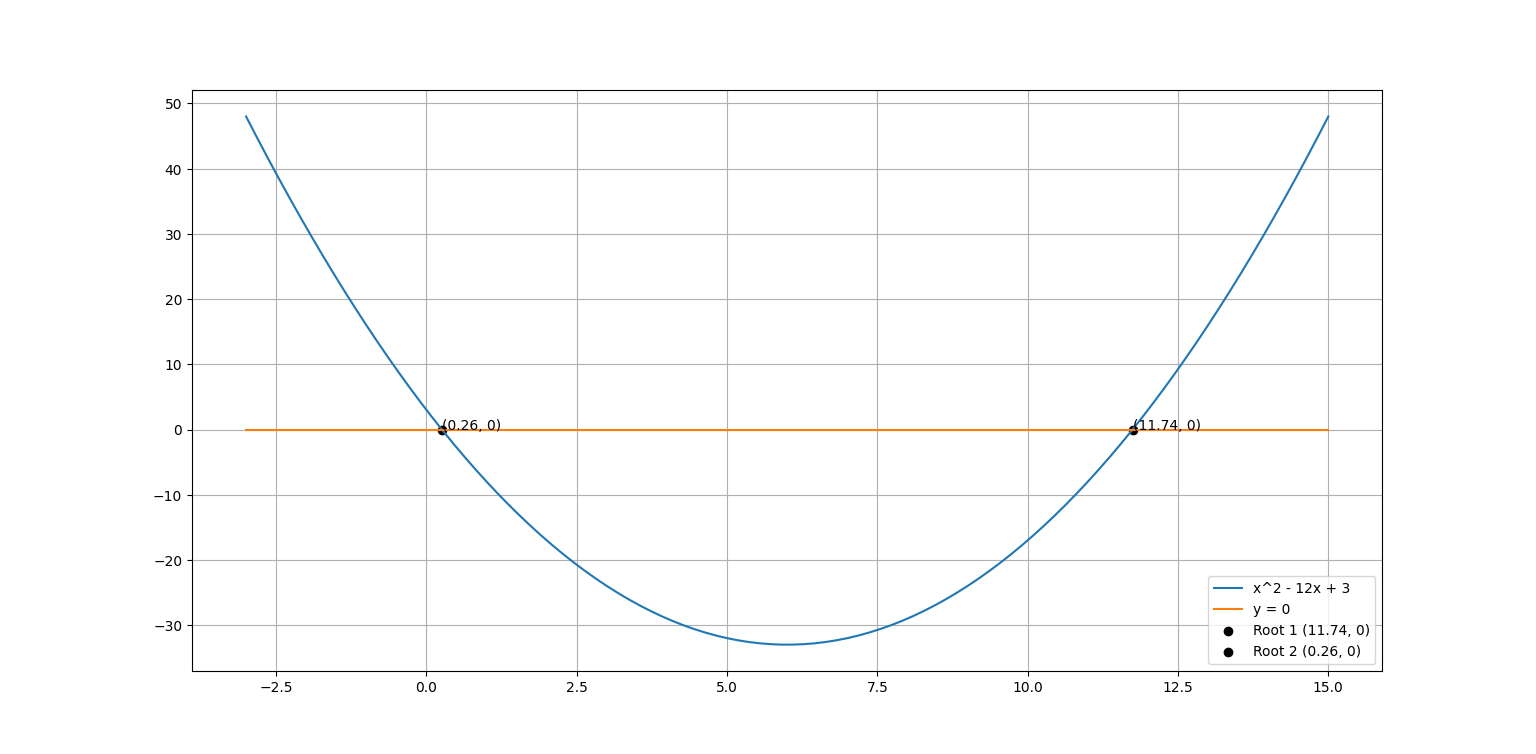
\includegraphics[width=\columnwidth]{figs/figure_py.png}
    \caption{Graph}
    \label{fig:fig}
 \end{figure}


\end{document}
